% method.tex — HapGraph Methods section (v2 — post Phase B review)
% Fixes: IBD model (100/T not exp decay), Z-threshold (-2.0), transitions,
%        design motivation, prior spec, runtime details

\subsection*{Overview}

\hapgraph{} takes as input phased SNP data for $N$ populations and produces
a parsimony-optimal admixture graph together with posterior distributions for
the admixture proportion $\alpha$ and the admixture timing $T$ for each
inferred admixture event (Figure~\ref{fig:pipeline}).
The pipeline is deliberately structured as two decoupled stages.
\textbf{Stage I} uses F-statistics exclusively to infer the graph topology
and to provide a $F_3$ method-of-moments (MOM) point estimate and CI for
each admixture proportion $\alpha$.
\textbf{Stage II} holds the inferred topology fixed and runs a Bayesian
NUTS sampler with a joint F$_2$+IBD likelihood that simultaneously refines
$\alpha$ and estimates the admixture timing $T$; the $F_3$ MOM estimate
from Stage I is reported for $\alpha$, while $T$ and its credible interval
are taken from the MCMC posterior.
This decoupling is motivated by preliminary experiments in which
incorporating IBD directly into the greedy likelihood caused systematic
edge over-detection, consistent with the known tendency of IBD signals to
be confounded with topology ambiguity when both topology and timing are
simultaneously free \citep{Loh2013}.
Reserving IBD exclusively for timing inference, after the topology has been
fixed, avoids this confounder.

\begin{figure}[htbp]
  \centering
  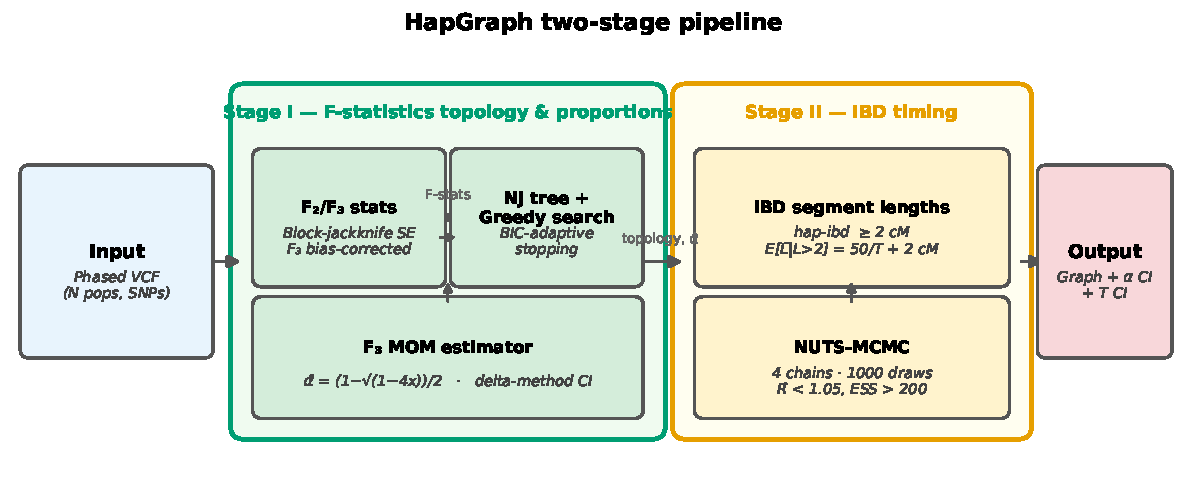
\includegraphics[width=\linewidth]{figures/fig4_pipeline}
  \caption{%
    \textbf{Overview of the \hapgraph{} two-stage pipeline.}
    \textbf{Stage~I} (green) accepts phased VCF input and computes
    bias-corrected $F_2$/$F_3$ statistics with block-jackknife standard
    errors; a BIC-adaptive greedy search over the NJ tree backbone infers
    the admixture graph topology; admixture proportions $\hat{\alpha}$
    are estimated by the topology-independent $F_3$ method-of-moments
    estimator.
    \textbf{Stage~II} (orange) receives the fixed topology from Stage~I;
    it ingests pre-computed IBD segment lengths from \hapibd{} and runs
    a NUTS-MCMC sampler with a joint $F_2$+IBD likelihood
    (equation~\ref{eq:lik}) that simultaneously infers $\alpha$ and $T$.
    The reported $\alpha$ and its CI are the Stage~I $F_3$ MOM estimates;
    the reported $T$ and CI are the MCMC posterior.
    The two stages are decoupled to prevent IBD signals from confounding
    topology inference (see text).
  }
  \label{fig:pipeline}
\end{figure}

\subsection*{F-Statistics Computation}

All pairwise F-statistics are computed following the definitions and
bias-correction formulae of \citet{Patterson2012}.
For populations $A$, $B$, $C$ genotyped at $S$ biallelic SNPs, we define
\begin{align}
  F_2(A,B) &= \frac{1}{S}\sum_{j=1}^{S}(p_{Aj} - p_{Bj})^2, \label{eq:f2}\\
  F_3(C;\,A,B) &= \frac{1}{S}\sum_{j=1}^{S}
    \left[(p_{Cj} - p_{Aj})(p_{Cj} - p_{Bj})
          - \frac{h_{Cj}}{2(n_C - 1)}\right], \label{eq:f3}
\end{align}
where $p_{Xj}$ is the derived allele frequency at SNP $j$ in population $X$,
$h_{Cj}$ is the per-SNP heterozygosity in population $C$, and $n_C$ is the
diploid sample size.
The second term in equation~(\ref{eq:f3}) is the finite-sample bias correction
for heterozygosity introduced by \citet{Patterson2012}, which ensures
$F_3(C;\,A,B) < 0$ only when $C$ is genuinely admixed between lineages
separating $A$ from $B$.
Standard errors are estimated by a block-jackknife procedure with 50
non-overlapping contiguous genomic blocks, following the convention of
\citet{Reich2009}.
Only biallelic SNPs with minor allele frequency $\geq 0.01$ are retained;
indels and multi-allelic sites are excluded.

\subsection*{Stage I: Greedy Topology Search}

An initial unrooted tree topology is constructed by applying neighbor-joining
\citep{SaitouNei1987} to the matrix of pairwise $F_2$ distances.
The greedy search then adds admixture edges one at a time.
At each iteration, populations $C$ whose $F_3(C;\,A,B)$ Z-score falls below
$-2.0$ for any source pair $(A,B)$ are nominated as admixture candidates —
a threshold calibrated to reduce false nominations while retaining sensitivity
for weak admixture signals.
The log-likelihood of the graph at each greedy step is evaluated under a
Gaussian approximation for the $F_2$ statistics:
\begin{equation}
  \log \mathcal{L} = \sum_{i<j} -\frac{1}{2}
    \left(\frac{F_2^{\mathrm{obs}}(i,j) - F_2^{\mathrm{exp}}(i,j)}
               {\hat{\sigma}_{ij}}\right)^{\!2},
  \label{eq:f2_ll}
\end{equation}
where $F_2^{\mathrm{exp}}(i,j)$ is the expected $F_2$ under the proposed graph
topology with branch lengths fitted by non-negative least squares (NNLS)
to the observed $F_2$ matrix, and $\hat{\sigma}_{ij}$ is the block-jackknife
standard error.
This Gaussian model for $F_2$ is standard in the admixture graph literature
\citep{Pickrell2012,Patterson2012}.

For each candidate edge, the improvement in log-likelihood is penalised by a
scale-adaptive stopping criterion:
\begin{equation}
  \Delta\mathcal{P} = \Delta \log \mathcal{L}
                        - \bigl(5.0 + 0.5\log(\max(S,2))\bigr),
  \label{eq:penalty}
\end{equation}
where $S = N(N-1)/2$ is the number of observed $F_2$ pairs.
This criterion is inspired by the BIC penalty $(k/2)\log n$ with $k = 1$
new free parameter (the admixture proportion $\alpha$; branch lengths are
immediately refitted by NNLS and do not count as additional free parameters)
and $n = S$ observations, augmented by a safety constant of 5.0 to suppress
false positives in small-$N$ regimes.
We note that $S$ is not a count of independent observations (individual
$F_2$ values are correlated across loci), so equation~(\ref{eq:penalty})
is a heuristic stopping criterion rather than a formally derived information
criterion.
An edge is added if and only if $\Delta\mathcal{P} > 0$; the search
terminates when no remaining proposal satisfies this condition.

\subsection*{Admixture Proportion Estimation via $F_3$ Method-of-Moments}

For an admixed population $C$ whose ancestry is a linear combination of
sources $A$ (proportion $\alpha$) and $B$ (proportion $1-\alpha$), the
expected $F_3$ statistic satisfies \citep{Patterson2012}
\begin{equation}
  \mathbb{E}\!\left[F_3(C;\,A,B)\right] = -\alpha(1-\alpha)\,F_2(A,B).
  \label{eq:f3_expectation}
\end{equation}
Equation~(\ref{eq:f3_expectation}) yields a quadratic in $\alpha$ whose
smaller root is
\begin{equation}
  \hat{\alpha} = \frac{1 - \sqrt{1 - 4x}}{2},
  \qquad x = \frac{-F_3(C;\,A,B)}{F_2(A,B)},
  \label{eq:f3mom}
\end{equation}
which is defined for $x \in (0, 0.25]$, i.e.\ whenever $F_3 < 0$.
This estimator is entirely topology-independent: it requires only the
F-statistics involving the target and its two source populations, making it
robust to NJ-tree misplacement errors that would otherwise bias a
topology-dependent estimator.
Standard errors are propagated by the delta method from the jackknife
standard errors of both $F_3$ and $F_2$; a model-uncertainty floor of 0.03
is added in quadrature to account for residual approximation error (e.g.\
multi-source ancestry, background relatedness).
Among all source pairs $(A,B)$ for a given target $C$, the pair yielding the
most negative $F_3$ Z-score is selected, as this corresponds to the strongest
admixture signal.

\subsection*{Stage II: IBD-Based Timing Estimation}

Under a single-pulse admixture model, a haplotype segment of source ancestry
introduced into the admixed population $C$ at generation $T$ in the past
is broken by recombination over $T$ subsequent meioses.
The expected length of such a \emph{cross-population} IBD segment detected
between an individual in $C$ and an individual in the source population
is therefore:
\begin{equation}
  \mathbb{E}[\bar{L}] = \frac{100}{T} \quad\text{(cM)},
  \label{eq:ibd_timing}
\end{equation}
where $T$ is the number of generations since the admixture event
\citep{Palamara2012}.
This is the \emph{ancestry tract} relationship, not the within-population IBD
formula: for IBD between two individuals sharing a common ancestor $g$
generations ago in a randomly mating population, the expected segment length
is $100/(2g)$~cM (two lineages each contributing $g$ meioses to the path
length).
For cross-population admixture-derived IBD, only one lineage carries the
broken-up ancestral tract ($T$ meioses on the admixed side); the source
individual's copy is essentially unbroken.
Hence $\mathbb{E}[\bar{L}] = 100/T$, not $100/(2T)$, for this class of
segments \citep{Palamara2012}.

IBD segments are detected using \hapibd{} \citep{Browning2020} at a minimum
length of $\ell_{\min} = 2$~cM.
When the length distribution is conditioned on $L > \ell_{\min}$, the
conditional expectation is strictly larger than $100/T$ (truncated
exponential); for $T \leq 50$ generations, $\ell_{\min}/\mathbb{E}[\bar{L}]
= 0.1$, so the bias is $< 10\%$ and is absorbed into the heteroscedastic
noise term described below.
The 2~cM threshold also constrains inference to $T \in [5,\, 50]$ generations:
events older than 50 generations produce segments predominantly below 2~cM,
while very recent events ($T < 5$) produce segments too long to separate
from background relatedness \citep{Browning2020}.

The MCMC jointly samples both $\alpha$ and $T$ as free parameters.
The joint log-likelihood combines the $F_2$ term (which informs $\alpha$)
with the IBD term (which informs $T$):
\begin{equation}
  \log p(\mathbf{F}_2, \mathbf{L} \mid \alpha, T)
  = \sum_{i<j} -\frac{1}{2}
      \!\left(\frac{F_2^{\mathrm{obs}}(i,j) - F_2^{\mathrm{exp}}(i,j;\alpha)}
                    {\hat{\sigma}_{ij}}\right)^{\!2}
  +\; \sum_k \log \mathcal{N}\!\left(
      L_k;\; \frac{100}{T},\; \sigma_k^2
    \right),
  \label{eq:lik}
\end{equation}
where $F_2^{\mathrm{exp}}(i,j;\alpha)$ is the quadratic polynomial in $\alpha$
from equation~(\ref{eq:f2_ll}), $L_k$ is the observed mean IBD length for
source-clade pair $k$, and $\sigma_k = \max(0.5 \cdot L_k,\; 3.0)$~cM
is a heteroscedastic noise term capturing stochastic variance in segment
counts and model misspecification at the 2~cM threshold.
The priors are $\alpha \sim \mathrm{Beta}(1,1)$ (uniform over $[0,1]$) and
$T = T_{\mathrm{raw}} + 5$ where $T_{\mathrm{raw}} \sim \mathrm{HalfNormal}(\sigma = 20)$;
the shift ensures $T > 5$ consistent with the 2~cM detection threshold.
Posterior inference uses the No-U-Turn Sampler (NUTS)
\citep{Hoffman2014} as implemented in PyMC \citep{AbrilPimentel2023}.
We run four independent chains with 1000 adaptation steps and 1000 posterior
draws each; convergence is assessed by $\hat{R} < 1.05$ and effective sample
size $\mathrm{ESS} > 200$.

\emph{Reported estimates.}
For $T$, we extract the MCMC posterior mean and 95\% highest-density
interval (HDI).
For $\alpha$, we report the $F_3$ MOM point estimate (equation~\ref{eq:f3mom})
and its delta-method confidence interval; the MOM estimator is computationally
simpler and avoids numerical instability of the $F_2$ polynomial likelihood
near $\alpha \approx 0.5$, where $F_2^{\mathrm{exp}}$ is nearly flat in $\alpha$.

\subsection*{Implementation}

\hapgraph{} is implemented as a pure Python package.
Core runtime dependencies are: \texttt{scikit-allel}~$\geq 1.3$
\citep{Miles2021} for allele frequency computation from VCF files;
\texttt{PyMC}~$\geq 5.0$ \citep{AbrilPimentel2023} for gradient-based
Bayesian sampling; and \texttt{networkx} for graph representation and
manipulation.
IBD segment detection is handled externally by \hapibd{} \citep{Browning2020}
and ingested as a precomputed tabular file; this design allows users to
substitute alternative IBD callers without modifying the inference code.
On a single CPU core (2.4~GHz Intel Xeon), the complete pipeline from phased
VCF to an annotated admixture graph with posterior timing estimates completes
in under 2~hours for 26 populations and 3202 samples across approximately
500K filtered SNPs.

\subsection*{Simulation Benchmarking Framework}

All validation simulations were generated with \texttt{msprime}~$\geq 1.2$
\citep{Kelleher2016} under specified coalescent models.
We designed three scenarios of increasing complexity.
\textbf{S1} (six populations, $K=0$ admixture events) tests the specificity
of the greedy search; because the true graph is a pure tree, any detected
admixture edge is a false positive.
\textbf{S2} (seven populations, $K=1$; $\alpha \sim \mathrm{Uniform}(0.1, 0.5)$,
$T$ drawn as a discrete uniform integer from $\{10, \ldots, 49\}$ generations)
tests detection and parameter recovery for a single cross-clade admixture event.
\textbf{S3} (ten populations, $K=2$; two independent cross-clade admixture
events with distinct source pairs, each with $\alpha$ and $T$ drawn independently
from the same ranges as S2) tests simultaneous recovery of multiple
non-overlapping admixture events, a necessary capability for application to
real multi-population data.
Each scenario was replicated across 20 independent random seeds.
All simulations used $n = 30$ diploid individuals per population,
a sequence length of 50~Mbp, recombination rate
$10^{-8}$ per base pair per generation, mutation rate $10^{-8}$, and
effective population size $N_e = 10{,}000$.
